% !TEX program = xelatex
\documentclass[aspectratio=169,10pt]{beamer}

\usepackage[UTF8,fontset=fandol]{ctex}
\usepackage{amsmath,amssymb,booktabs,tabularx,multirow}
\usepackage{graphicx,tikz}
\usetikzlibrary{positioning,arrows.meta,calc,fit}
\usepackage{CUHKBeamer}

\title[EgoMimic × VidBot]{从人类视频到机器人动作}
\subtitle{EgoMimic 与 VidBot：方法、证据与复现进展}
\author[具身智能文献汇报]{汇报人：\underline{\hspace{3.0cm}}}
\institute[文献与复现实验]{具身智能文献与复现实验汇报}
\date{2026年9月}

\newcommand{\src}[1]{\vfill{\fontsize{5.8}{6.8}\selectfont\color{CUHKMidGray}来源：#1}}
\newcommand{\takeaway}[1]{\begin{beamercolorbox}[rounded=true,sep=.52em,wd=\linewidth]{block body alerted}\textcolor{CUHKDeepPurple}{\bfseries 结论}\quad #1\end{beamercolorbox}}
\newcommand{\tagbox}[1]{\tikz[baseline=(X.base)]\node[fill=CUHKPurple!10,draw=CUHKPurple,rounded corners=1.5pt,inner xsep=4pt,inner ysep=2pt] (X) {\scriptsize #1};}
\setbeamertemplate{caption}{\raggedright\insertcaption\par}

\begin{document}

{
\setbeamercolor{background canvas}{bg=CUHKPurple}
\begin{frame}[plain]
  \titlepage
\end{frame}
}

\begin{frame}{汇报路线}
  \tableofcontents
  \vspace{.25cm}
  \takeaway{两篇论文共享同一目标：降低机器人示教成本；但学习目标不同——EgoMimic 学策略，VidBot 学可迁移的 3D 交互轨迹。}
\end{frame}

\section{问题与基础概念}

\begin{frame}{共同问题：机器人数据昂贵，人类视频丰富}
  \begin{columns}[T,onlytextwidth]
    \begin{column}{.48\textwidth}
      \begin{block}{EgoMimic}
        \textbf{输入：}第一人称人手数据 + 机器人示教\\[3pt]
        \textbf{输出：}可直接预测机器人动作的联合策略\\[3pt]
        \textbf{关键词：}跨域对齐、共享表征、多头监督
      \end{block}
    \end{column}
    \begin{column}{.48\textwidth}
      \begin{block}{VidBot}
        \textbf{输入：}网络中的普通单目人类视频 + 语言\\[3pt]
        \textbf{输出：}接触点与 3D 末端轨迹\\[3pt]
        \textbf{关键词：}SfM、深度、可供性、扩散轨迹
      \end{block}
    \end{column}
  \end{columns}
  \vspace{.35cm}
  \centering
  \begin{tikzpicture}[node distance=.6cm, every node/.style={align=center}]
    \node[draw,rounded corners,fill=CUHKSoftGray,minimum width=2.5cm,minimum height=.75cm] (h) {人类行为数据\\\scriptsize 便宜、多样、但非机器人域};
    \node[draw,rounded corners,fill=CUHKPaleGold,minimum width=2.5cm,minimum height=.75cm,right=of h] (r) {可迁移动作表征\\\scriptsize pose / contact / trajectory};
    \node[draw,rounded corners,fill=CUHKSoftGray,minimum width=2.5cm,minimum height=.75cm,right=of r] (p) {机器人执行\\\scriptsize policy 或规划控制};
    \draw[-{Latex},very thick,CUHKGold] (h)--(r);
    \draw[-{Latex},very thick,CUHKGold] (r)--(p);
  \end{tikzpicture}
\end{frame}

\section{EgoMimic：人机数据联合策略学习}

\begin{frame}{EgoMimic 方法总览}
  \centering
  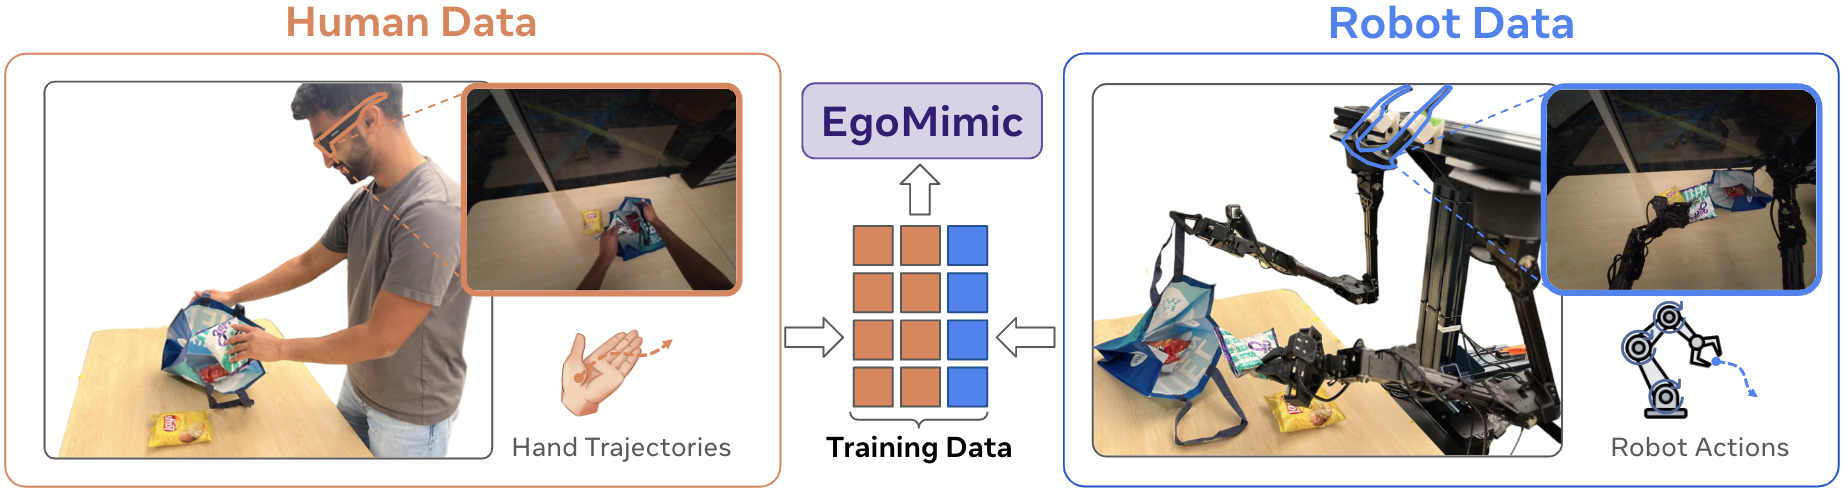
\includegraphics[width=.90\textwidth,height=.52\textheight,keepaspectratio]{assets/egomimic_overview.png}
  \vspace{.18cm}
  \resizebox{.94\textwidth}{!}{\begin{tikzpicture}[node distance=.32cm,box/.style={draw=CUHKPurple,rounded corners=2pt,fill=CUHKSoftGray,minimum height=.54cm,align=center,font=\scriptsize},arr/.style={-{Latex},thick,CUHKGold}]
    \node[box] (a) {人：Aria RGB + 3D 手};
    \node[box,right=of a] (b) {机：RGB + 关节 + EE};
    \node[box,right=of b] (c) {坐标/速度/分布/视觉对齐};
    \node[box,right=of c] (d) {共享 ACT 主干 + 域专属头};
    \node[box,right=of d] (e) {机器人动作 chunk};
    \draw[arr] (a)--(c); \draw[arr] (b)--(c); \draw[arr] (c)--(d); \draw[arr] (d)--(e);
  \end{tikzpicture}}
  \src{Kareer et al., \textit{EgoMimic}, 2024, Fig. 1.}
\end{frame}

\begin{frame}{人类数据与机器人数据的原始差异}
  \small
  \begin{columns}[T,onlytextwidth]
    \begin{column}{.49\textwidth}
      \centering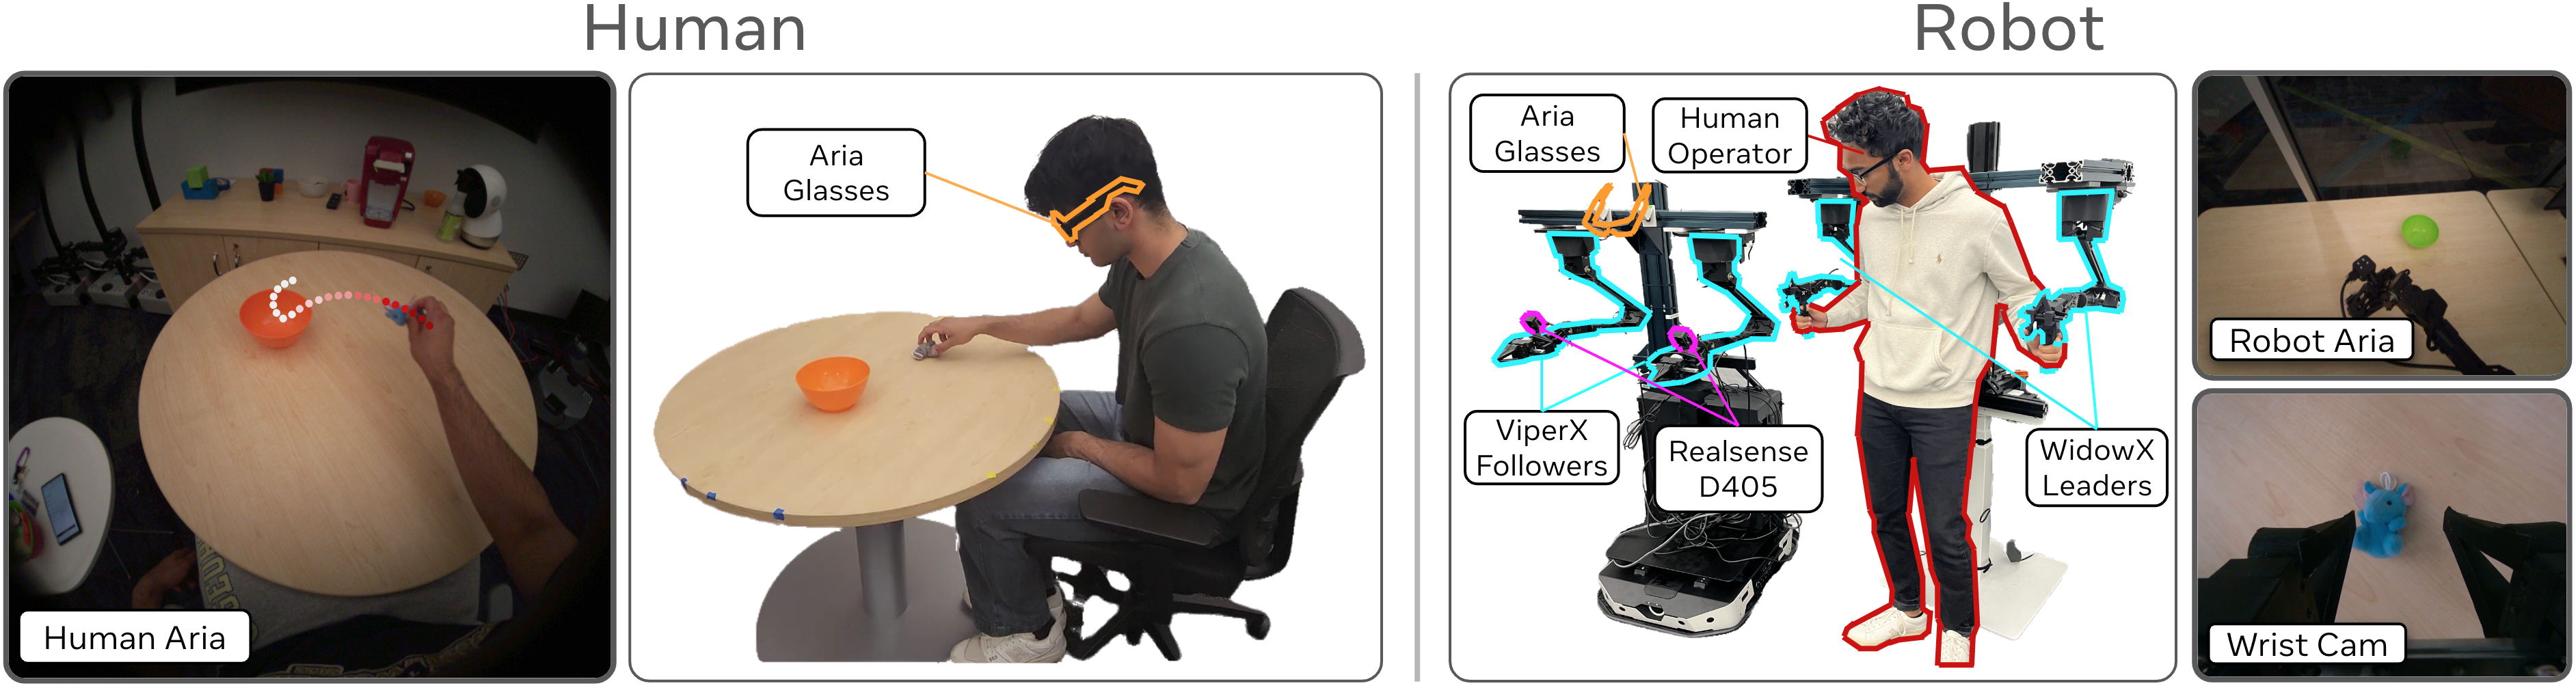
\includegraphics[width=\linewidth,height=.34\textheight,keepaspectratio]{assets/egomimic_hardware.png}
    \end{column}
    \begin{column}{.49\textwidth}
      \begin{tabularx}{\linewidth}{lXX}
        \toprule
        差异 & 人类域 & 机器人域\\
        \midrule
        形态 & 手/身体 & 连杆/夹爪\\
        状态 & 3D 手位姿 & 关节、EE、夹爪\\
        视角 & 头戴相机 & 顶视 + 腕部相机\\
        速度 & 快、自然 & 慢、受控制约束\\
        外观 & 手遮挡 & 机械臂遮挡\\
        \bottomrule
      \end{tabularx}
    \end{column}
  \end{columns}
  \vspace{.25cm}
  \takeaway{不能把两个 HDF5 简单拼接：至少要解决“同一个动作如何表达、同一个场景如何看起来相近、缺失字段由谁监督”。}
  \src{Kareer et al., 2024, Sec. III-B/C；项目数据字段与加载代码。}
\end{frame}

\begin{frame}{跨域对齐：把“可共享部分”映射到同一语义}
  \scriptsize
  \begin{columns}[T,onlytextwidth]
    \begin{column}{.50\textwidth}
      \begin{block}{1. 坐标系对齐}
        人手未来位置通过 Aria MPS/SLAM 变换到\textbf{当前相机坐标系}；机器人 EE 由 FK + 手眼标定得到相机坐标。
        \[
          {}^{C_t}\!p_{t+k}=T_{C_t\leftarrow W}\,T_{W\leftarrow C_{t+k}}\,{}^{C_{t+k}}\!p_{t+k}
        \]
      \end{block}
      \begin{block}{2. 时间对齐}
        同为 100 个未来点：人类覆盖约 1 s，机器人覆盖约 4 s，相当于把人手运动“放慢”到机器人节奏。
      \end{block}
    \end{column}
    \begin{column}{.46\textwidth}
      \begin{block}{3. 数值分布对齐}
        每个域分别做 Gaussian / Z-score 归一化：
        \[
          \tilde a^{(d)}=(a^{(d)}-\mu_d)/(\sigma_d+\epsilon)
        \]
        避免一个域的量纲和方差支配梯度。
      \end{block}
      \begin{alertblock}{“对齐”不等于数据完全相同}
        共享的是\textbf{末端运动语义}；机器人关节、夹爪、腕部图像仍保留为机器人专属信号。
      \end{alertblock}
    \end{column}
  \end{columns}
  \src{Kareer et al., 2024, Sec. III-C；Supplementary Sec. VI.}
\end{frame}

\begin{frame}{视觉外观对齐：mask 掉 embodiment，再保留运动方向}
  \begin{columns}[c,onlytextwidth]
    \begin{column}{.58\textwidth}
      \centering
      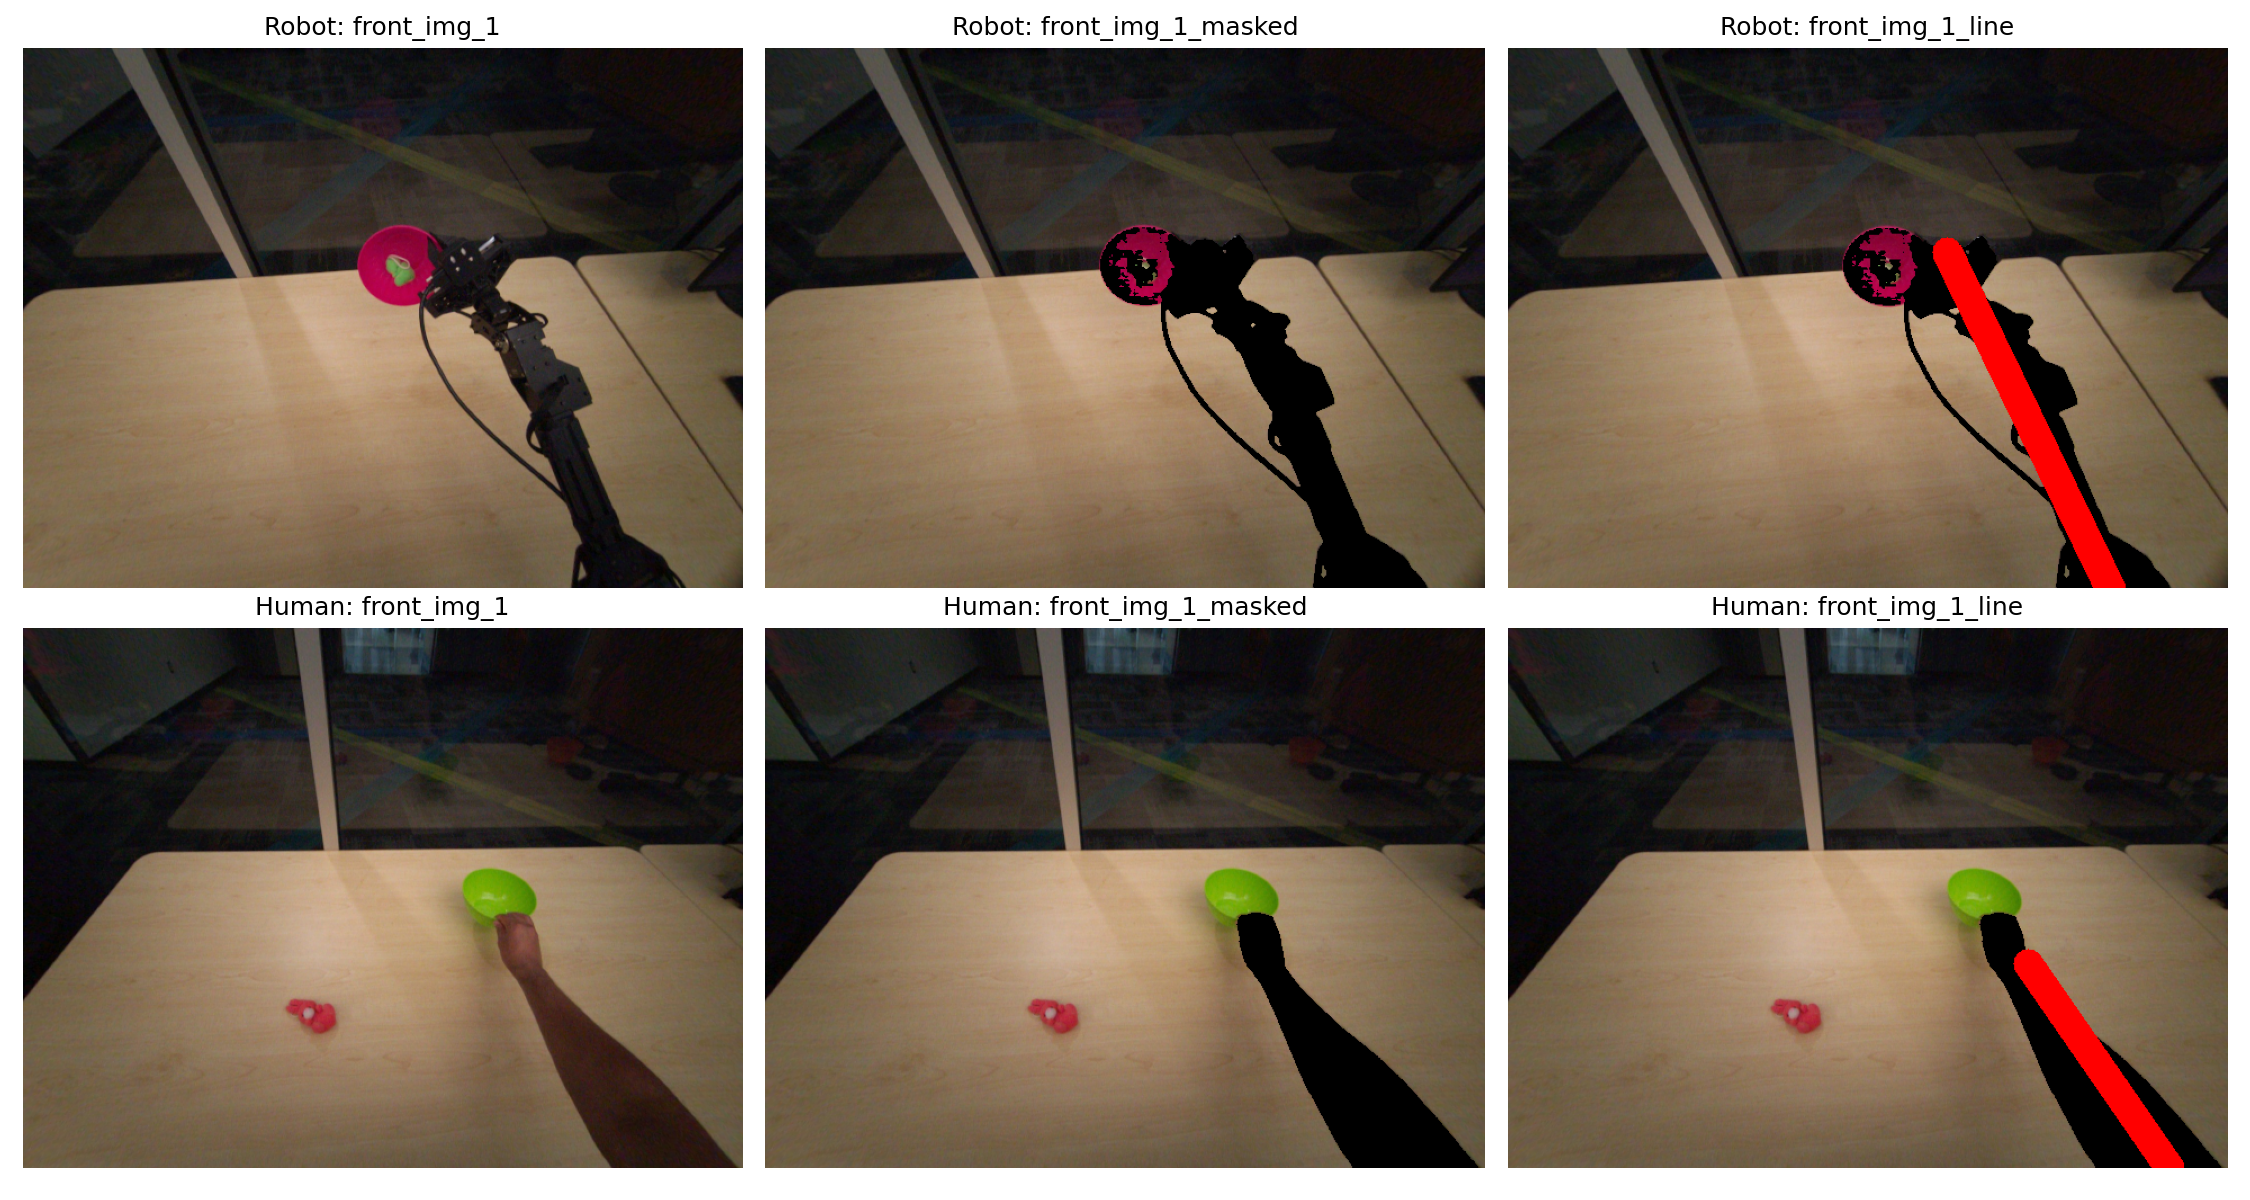
\includegraphics[width=\linewidth,height=.62\textheight,keepaspectratio]{assets/local_mask_comparison.png}
      
      {\scriptsize 你下载的数据：human / robot 原图、mask 与对齐后输入}
    \end{column}
    \begin{column}{.38\textwidth}
      \small
      \begin{enumerate}
        \item SAM2 分割人手或机械臂；
        \item 将实体区域遮蔽，减小形态与纹理差异；
        \item 叠加红色方向线，避免把与动作有关的信息全部删掉。
      \end{enumerate}
      \vspace{.2cm}
      \begin{alertblock}{mask 与动作线索的平衡}
        消融中去掉方向线、进一步去掉 mask，性能继续下降；视觉对齐既要“去域差异”，也要“留动作线索”。
      \end{alertblock}
    \end{column}
  \end{columns}
  \src{本地 bowlplace 数据可视化；Kareer et al., 2024, Fig. 4 与 Table IV.}
\end{frame}

\begin{frame}{统一策略架构：共享主干 + 域专属输入/输出头}
  \begin{columns}[c,onlytextwidth]
    \begin{column}{.54\textwidth}
      \centering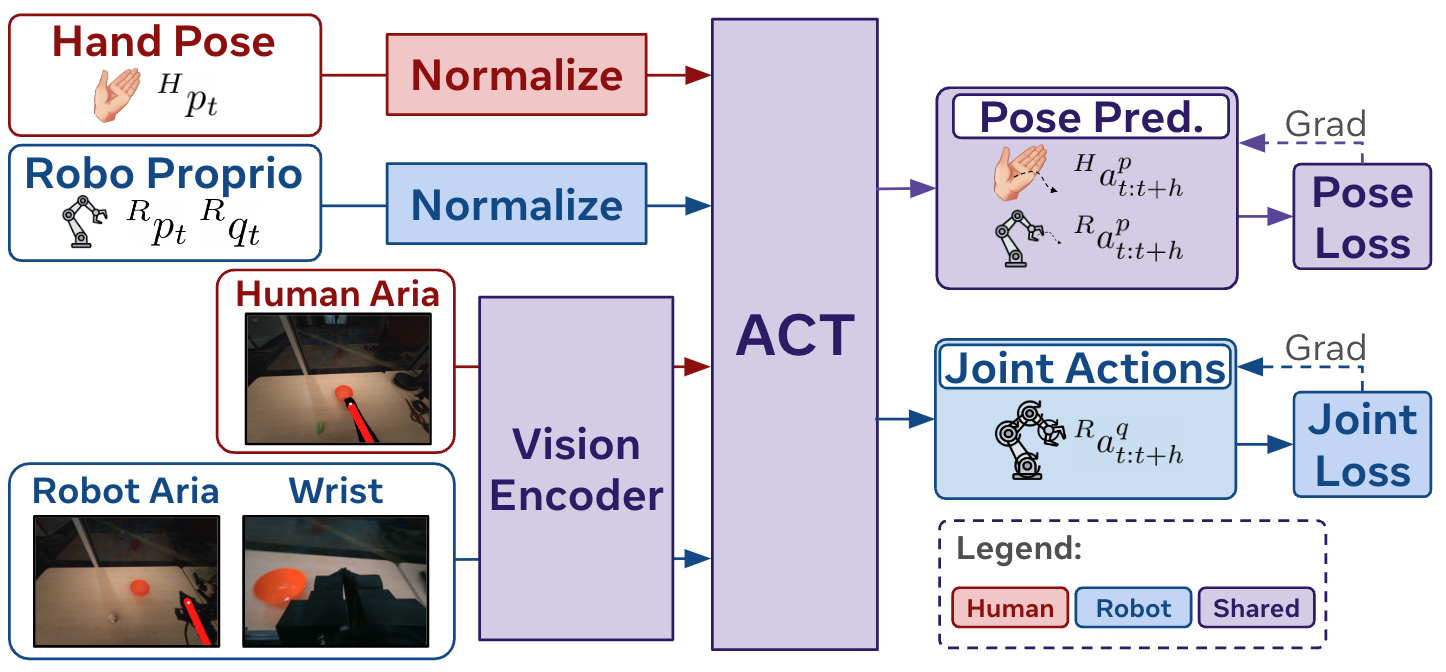
\includegraphics[width=\linewidth,height=.60\textheight,keepaspectratio]{assets/egomimic_arch.png}
    \end{column}
    \begin{column}{.43\textwidth}
      \small
      \begin{block}{共享}
        前视 RGB 编码器（ResNet18）与 ACT Transformer：共同学习“场景—目标—运动”的规律。
      \end{block}
      \begin{block}{域专属}
        输入投影与输出头不同；机器人额外使用腕部图像、关节和夹爪监督。
      \end{block}
      \begin{align*}
        \mathcal L_R &= \|\hat a_R^{pose}-a_R^{pose}\|_1\\
        &+\|\hat a_R^{joint}-a_R^{joint}\|_1+\mathrm{KL},\\
        \mathcal L_H &= \|\hat a_H^{pose}-a_H^{pose}\|_1+\mathrm{KL}.
      \end{align*}
    \end{column}
  \end{columns}
  \src{Kareer et al., 2024, Fig. 5；项目 \texttt{algo/act.py} 与双数据加载逻辑。}
\end{frame}

\begin{frame}{人机数据联合训练过程}
  \small
  \centering
  \resizebox{.86\textwidth}{!}{\begin{tikzpicture}[node distance=.52cm, box/.style={draw=CUHKPurple,rounded corners,fill=CUHKSoftGray,minimum height=.65cm,minimum width=2.0cm,align=center}, arr/.style={-{Latex},very thick,CUHKGold}]
    \node[box] (rb) {Robot batch\\\scriptsize RGB, wrist, $q$, EE, gripper};
    \node[box,below=of rb] (hb) {Human batch\\\scriptsize RGB, hand pose};
    \node[box,right=1.25cm of rb,yshift=-.57cm] (enc) {域专属投影\\+ 共享编码器};
    \node[box,right=of enc] (act) {共享 ACT\\Transformer};
    \node[box,right=of act,yshift=.45cm] (rh) {Robot heads\\\scriptsize pose + joint/gripper};
    \node[box,right=of act,yshift=-.45cm] (hh) {Human head\\\scriptsize pose};
    \draw[arr] (rb)--(enc); \draw[arr] (hb)--(enc); \draw[arr] (enc)--(act); \draw[arr] (act)--(rh); \draw[arr] (act)--(hh);
  \end{tikzpicture}}
  \vspace{.35cm}
  \begin{columns}[T,onlytextwidth]
    \begin{column}{.48\textwidth}
      \begin{block}{共同梯度}
        两域损失在同一优化步骤内汇总（代码中做平均），一起更新共享视觉与 Transformer 参数。
      \end{block}
    \end{column}
    \begin{column}{.48\textwidth}
      \begin{block}{缺失维度}
        人类没有关节/夹爪标签：\textbf{不填假值、不计算对应损失}；这些头只由机器人 batch 学习。
      \end{block}
    \end{column}
  \end{columns}
  \src{EgoMimic 开源实现：双 DataLoader / training step / ACT policy wrapper。}
\end{frame}

\begin{frame}{全机器人、人类与混合数据的实验对比}
  \begin{columns}[c,onlytextwidth]
    \begin{column}{.49\textwidth}
      \centering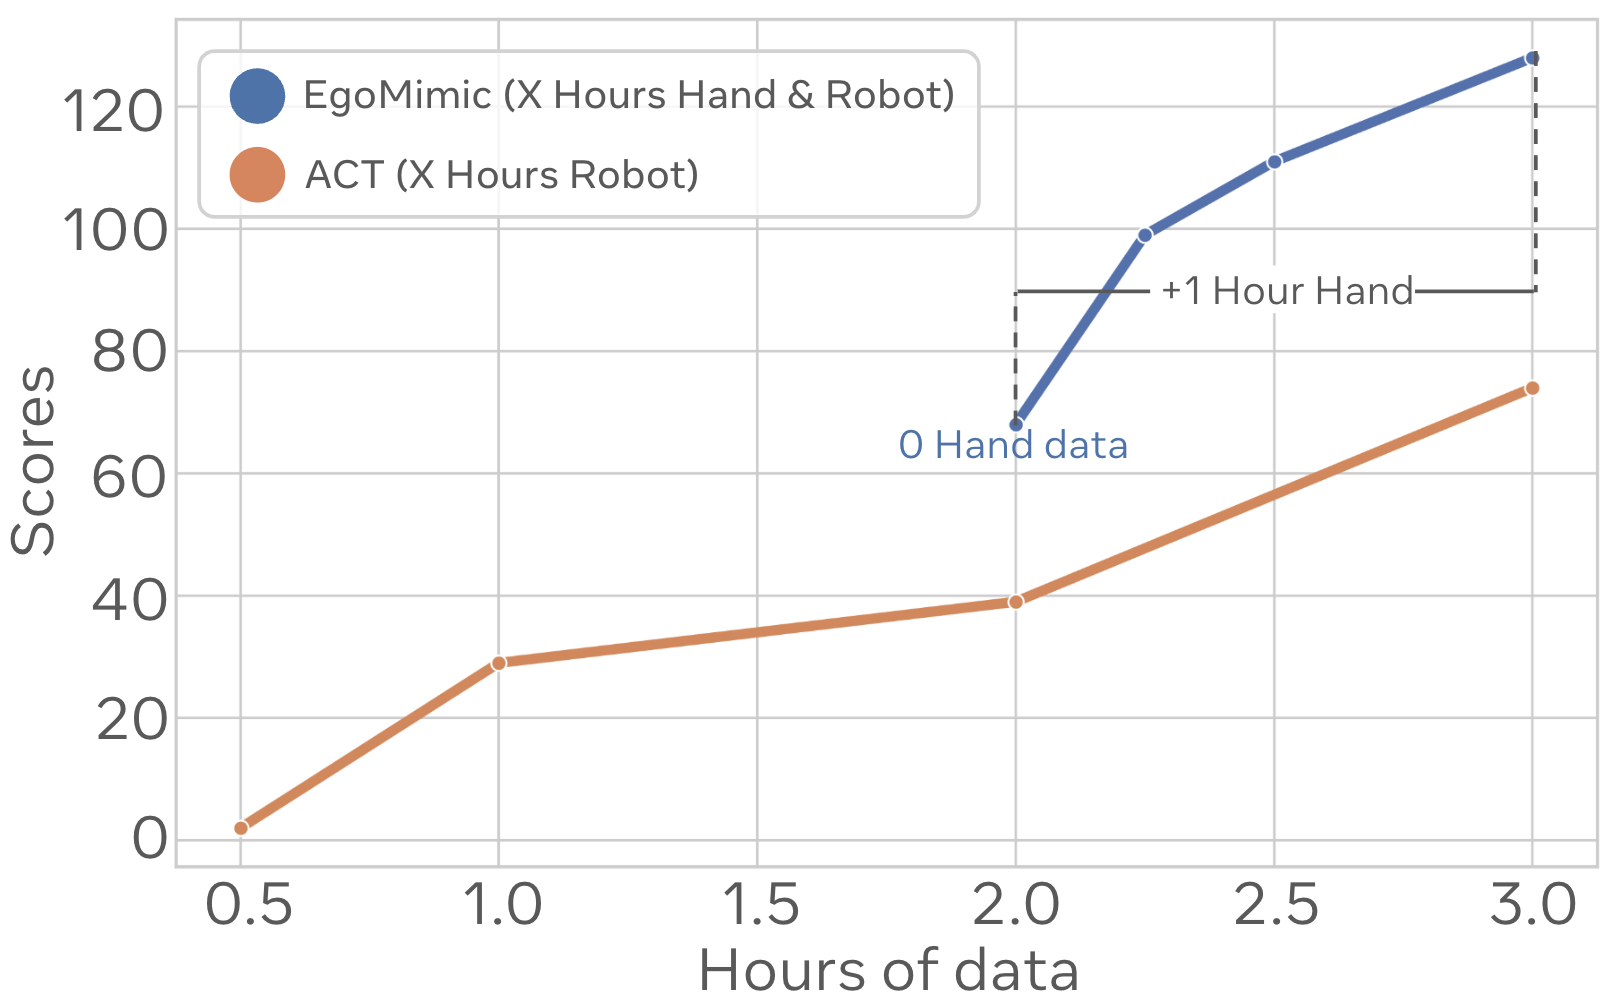
\includegraphics[width=\linewidth,height=.58\textheight,keepaspectratio]{assets/egomimic_scaling.png}
    \end{column}
    \begin{column}{.47\textwidth}
      \small
      \begin{alertblock}{论文采用的比较方式}
        \textbf{等采集时间}比较：2 h robot + 1 h human 的 EgoMimic 得分 128；3 h robot 的 ACT 得分 74。
      \end{alertblock}
      \begin{block}{论文未覆盖的严格对照}
        没有“相同轨迹条数”的全机器人 / 全人 / 混合三方对比；且纯人类数据缺少机器人关节与夹爪监督，不能直接构成完整部署策略。
      \end{block}
      \begin{block}{合理的控制组}
        EgoMimic w/o Human 保持架构不变，只去掉人类数据，用于隔离人类数据的增益。
      \end{block}
    \end{column}
  \end{columns}
  \src{Kareer et al., 2024, Fig. 8、Table II/III。1 h human 约 1400 条，1 h robot 约 135 条，因此“等时间”并非“等条数”。}
\end{frame}

\begin{frame}{论文证据：各模块对性能的贡献}
  \small
  \begin{columns}[T,onlytextwidth]
    \begin{column}{.54\textwidth}
      \centering
      \scriptsize
      \setlength{\tabcolsep}{3pt}
      \begin{tabular}{lrrr}
        \toprule
        方法 & Bowl 得分 & Laundry SR & Grocery SR\\
        \midrule
        ACT & 39 & 55\% & 22\%\\
        MimicPlay & 71 & 50\% & 8\%\\
        EgoMimic w/o H & 68 & 73\% & 28\%\\
        \textbf{EgoMimic} & \textbf{128} & \textbf{88\%} & \textbf{30\%}\\
        \bottomrule
      \end{tabular}
      \vspace{.35cm}
      \begin{tabular}{lr}
        \toprule
        Bowl 消融 & 得分\\
        \midrule
        Full / 去线 / 再去 mask & 128 / 112 / 95\\
        再去 action norm / 去 human & 79 / 68\\
        \bottomrule
      \end{tabular}
    \end{column}
    \begin{column}{.42\textwidth}
      \begin{block}{创新点不是单一模块}
        \begin{enumerate}
          \item 可扩展的人类第一视角采集；
          \item 面向人机共享的动作与视觉对齐；
          \item 共享策略主干 + 域专属头；
          \item 在长时程、双臂任务中验证规模效应。
        \end{enumerate}
      \end{block}
    \end{column}
  \end{columns}
  \src{Kareer et al., 2024, Table III/IV。指标定义因任务而异，勿横向混成同一“准确率”。}
\end{frame}

\begin{frame}{EgoMimic 复现}
  \begin{columns}[c,onlytextwidth]
    \begin{column}{.47\textwidth}
      \centering
      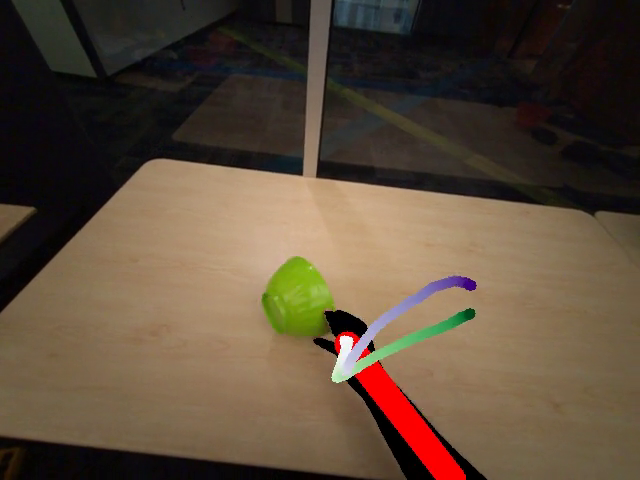
\includegraphics[width=.48\linewidth]{assets/local_hand_prediction.png}\hfill
      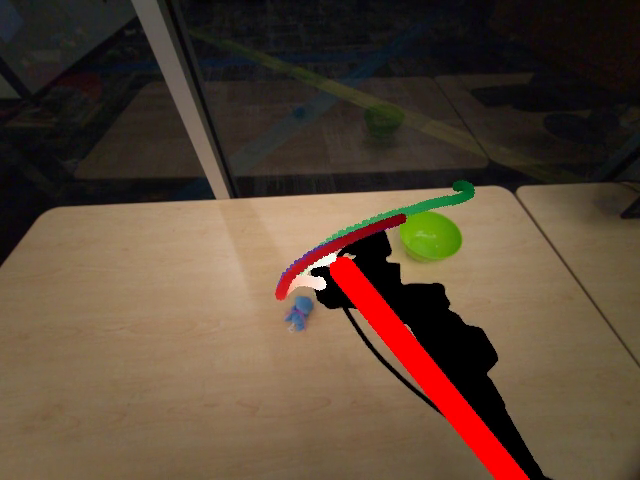
\includegraphics[width=.48\linewidth]{assets/local_robot_prediction.png}\\[4pt]
      {\scriptsize 左：人类域；右：机器人域}
      \vspace{.28cm}
      
      \begin{beamercolorbox}[rounded=true,sep=.45em,wd=\linewidth]{block body}
        \scriptsize
        \textcolor{green!55!black}{\bfseries 绿色：}真实未来轨迹\quad
        \textcolor{CUHKPurple}{\bfseries 紫色：}模型预测\\
        \textcolor{red!75!black}{\bfseries 红色：}机器人末端位姿预测头
      \end{beamercolorbox}
    \end{column}
    \begin{column}{.49\textwidth}
      \small
      \begin{block}{结果}
        \begin{itemize}
          \item 训练正常完成，human 与 robot 两个域均能生成连续未来轨迹；
          \item 从首次验证到最后一次验证，paired MSE 分别下降约 \textbf{25.4\%} 和 \textbf{23.1\%}；
          \item 两个域的最低验证误差均出现在约 epoch 400，随后略有回升。
        \end{itemize}
      \end{block}
      \begin{alertblock}{结果分析}
        预测已经捕捉到主要运动方向，短期轨迹通常与真实轨迹接近。偏差主要出现在长预测段和终点，部分样本呈现平滑化或平均化。后续闭环测试应优先比较 epoch 399 与最终 checkpoint。
      \end{alertblock}
    \end{column}
  \end{columns}
  \src{本地验证代码与第 50--450 轮验证日志；MSE 数值仅用于同一域内纵向比较。}
\end{frame}

\section{VidBot：从野外视频提取 3D 交互轨迹}

\begin{frame}{VidBot：把视频变成机器人可消费的 3D 动作}
  \centering
  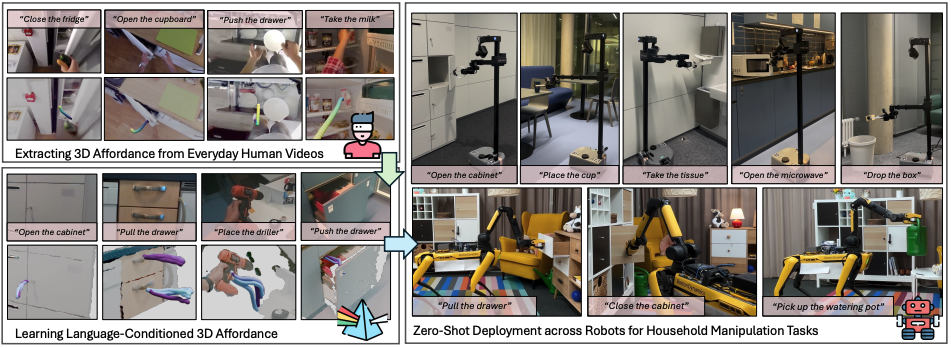
\includegraphics[width=.96\textwidth,height=.54\textheight,keepaspectratio]{assets/vidbot_teaser.png}
  \vspace{.2cm}
  \begin{columns}[T,onlytextwidth]
    \begin{column}{.48\textwidth}
      \begin{block}{训练时学习}
        从普通人类视频恢复 $a=\{c,\tau\}$：3D 接触点 $c$ 与交互轨迹 $\tau$。
      \end{block}
    \end{column}
    \begin{column}{.48\textwidth}
      \begin{block}{测试时执行}
        给机器人 RGB-D 场景与语言指令，生成候选 3D 轨迹，再交给 IK / 规划 / 控制执行。
      \end{block}
    \end{column}
  \end{columns}
  \src{Chen et al., \textit{VidBot: Learning Generalizable 3D Actions from In-the-Wild 2D Human Videos}, CVPR 2025, Fig. 1.}
\end{frame}

\begin{frame}{数据准备：单目 RGB 获得 3D 监督}
  \centering
  \begin{tikzpicture}[node distance=.26cm, box/.style={draw=CUHKPurple,rounded corners=2pt,fill=CUHKSoftGray,minimum width=1.72cm,minimum height=.72cm,align=center,font=\scriptsize}, arr/.style={-{Latex},thick,CUHKGold}]
    \node[box] (v) {人类单目视频\\+ 语言};
    \node[box,right=of v] (sfm) {SfM / COLMAP\\$K,\,T_t,\,P_{sparse}$};
    \node[box,right=of sfm] (dep) {单目度量深度\\$D_t^{metric}$};
    \node[box,right=of dep] (mask) {手/物体检测分割\\mask + inpainting};
    \node[box,right=of mask] (opt) {一致位姿优化\\尺度 + pose};
    \node[box,right=of opt] (traj) {统一到第0帧\\$c,\tau$};
    \draw[arr] (v)--(sfm); \draw[arr] (sfm)--(dep); \draw[arr] (dep)--(mask); \draw[arr] (mask)--(opt); \draw[arr] (opt)--(traj);
  \end{tikzpicture}
  \vspace{.35cm}
  \begin{columns}[T,onlytextwidth]
    \begin{column}{.48\textwidth}
      \begin{block}{SfM 的作用}
        Structure from Motion：利用多帧特征匹配同时估计相机内参/位姿与稀疏三维点。它提供\textbf{跨帧几何关系}，但整体尺度不确定。
      \end{block}
    \end{column}
    \begin{column}{.48\textwidth}
      \begin{block}{度量深度来源}
        使用预训练的 metric depth 模型得到每帧稠密深度；它补足尺度与稠密几何，但逐帧预测会有时间不一致。
      \end{block}
    \end{column}
  \end{columns}
  \src{Chen et al., 2025, Sec. III-B；其数据来源基于 EPIC-KITCHENS-100 / EPIC Fields 的预计算 SfM。}
\end{frame}

\begin{frame}{一致位姿优化：SfM 与深度的再对齐}
  \begin{columns}[c,onlytextwidth]
    \begin{column}{.47\textwidth}
      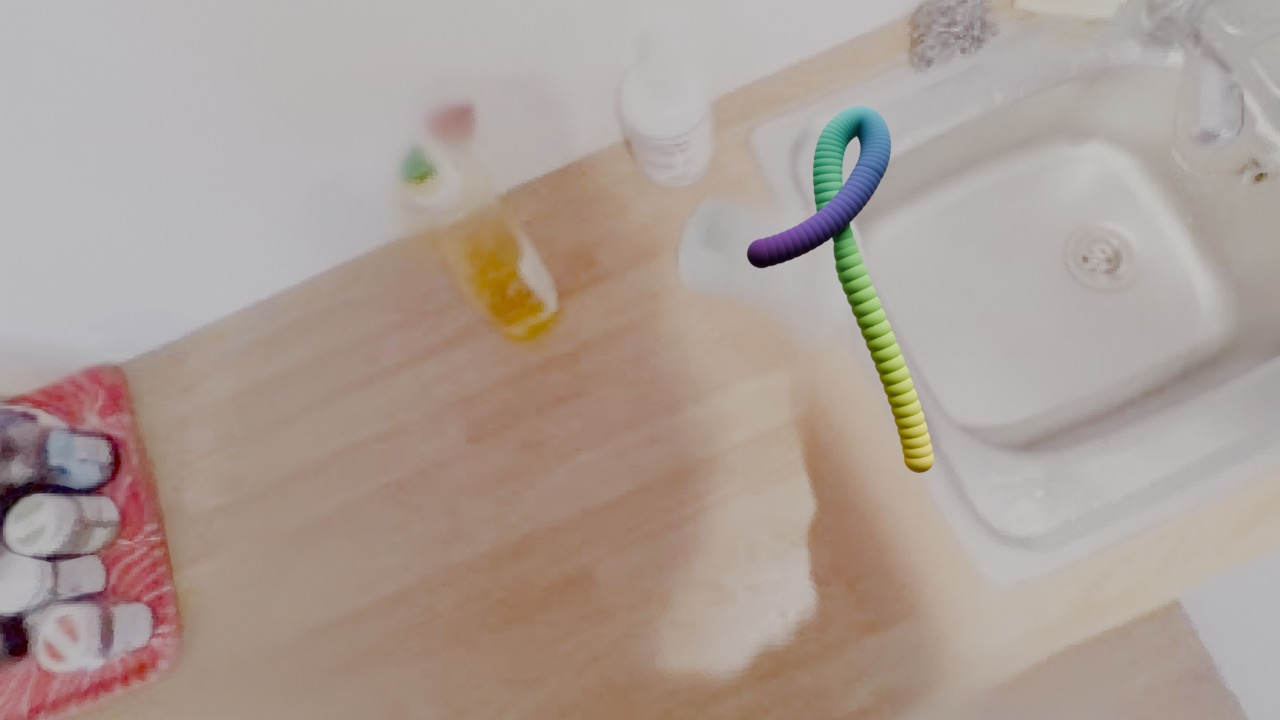
\includegraphics[width=\linewidth,height=.225\textheight,keepaspectratio]{assets/vidbot_traj_1.png}
      \vspace{.1cm}
      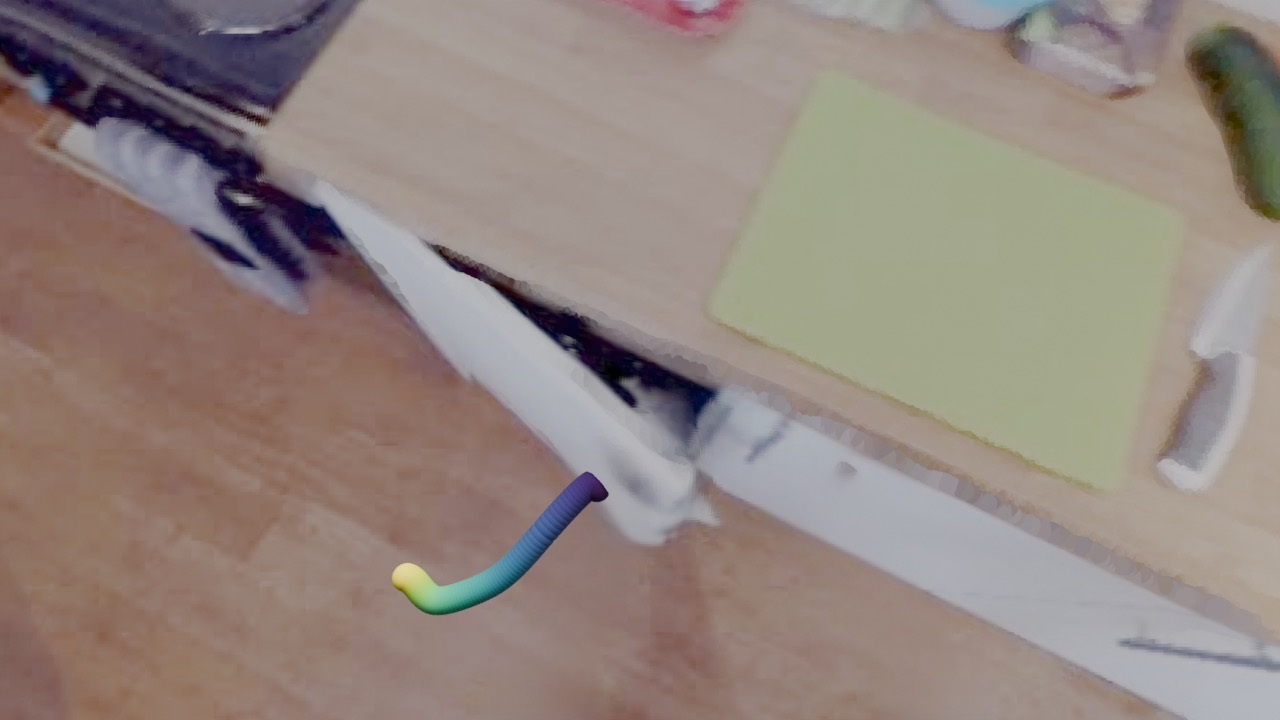
\includegraphics[width=\linewidth,height=.225\textheight,keepaspectratio]{assets/vidbot_traj_2.png}
    \end{column}
    \begin{column}{.49\textwidth}
      \small
      \begin{enumerate}
        \item 用静态背景点比较 SfM 深度与 metric depth，估计全局尺度；
        \item 再优化逐帧相机 pose 与深度尺度，使静态场景跨帧一致；
        \item 从每帧手 mask 求手中心像素 $(u_t,v_t)$，结合深度反投影成 3D；
        \item 用优化后的位姿把所有点变换到第 0 帧：
      \end{enumerate}
      \[
        p_t^{C_0}=T_{C_0\leftarrow W}\,T_{W\leftarrow C_t}
        \bigl(D_t(u_t,v_t)K^{-1}[u_t,v_t,1]^\top\bigr).
      \]
      \begin{alertblock}{核心}
        相机在动，但任务轨迹需要一个稳定参考系；因此“统一到第 0 帧”是在消除相机自身运动。
      \end{alertblock}
    \end{column}
  \end{columns}
  \src{Chen et al., 2025, Fig. 2 与 Sec. III-B。}
\end{frame}

\begin{frame}{三维可供性的粗细两阶段模型}
  \centering
  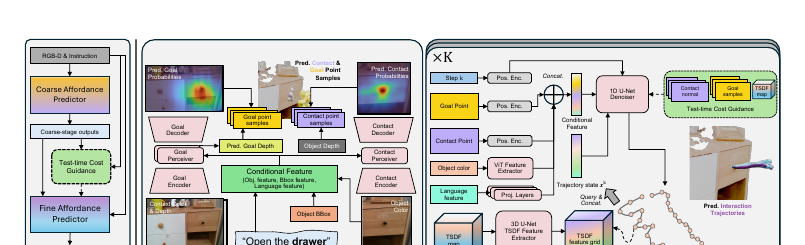
\includegraphics[width=.92\textwidth,height=.42\textheight,keepaspectratio]{assets/vidbot_method.png}
  \vspace{.15cm}
  \begin{columns}[T,onlytextwidth]
    \begin{column}{.48\textwidth}
      \begin{block}{粗可供性模型：接触点与目标点}
        视觉 + 语言预测 2D contact / goal 概率图；接触点深度可从物体表面读取，而 goal 可能在自由空间，因此额外预测 goal depth。
      \end{block}
    \end{column}
    \begin{column}{.48\textwidth}
      \begin{block}{细可供性模型：完整交互轨迹}
        1D U-Net 扩散模型以接触、目标、语言、物体特征和 TSDF 场景特征为条件，生成完整 3D 轨迹 $\tau$。
      \end{block}
    \end{column}
  \end{columns}
  \src{Chen et al., 2025, Fig. 3 与 Sec. III-C。}
\end{frame}

\begin{frame}{Language 条件与测试时轨迹筛选}
  \small
  \begin{columns}[T,onlytextwidth]
    \begin{column}{.48\textwidth}
      \begin{block}{语言条件}
        指令如 “\textit{open the microwave}” 经 CLIP 编码：
        \begin{itemize}
          \item 条件化 contact / goal 热图；
          \item 条件化扩散轨迹；
          \item 动词与物体名帮助选择检测目标及交互类型。
        \end{itemize}
      \end{block}
      \begin{alertblock}{语言条件的必要性}
        同一物体可能对应打开、关闭、拉出、放入；图像只告诉“有什么”，语言补充“要做什么”。
      \end{alertblock}
    \end{column}
    \begin{column}{.48\textwidth}
      \begin{block}{可微 guidance + 排序}
        扩散采样时施加：
        \begin{itemize}
          \item multi-goal：保留多种可能终点；
          \item collision：轨迹避开 TSDF 障碍；
          \item contact-normal：接近方向符合表面法向。
        \end{itemize}
        最终用综合代价从候选轨迹中选择一条。
      \end{block}
      \[
        \tau^*=\arg\min_{\tau_i}\bigl(\lambda_cJ_{coll}+\lambda_nJ_{normal}+\lambda_gJ_{goal}\bigr).
      \]
    \end{column}
  \end{columns}
  \src{Chen et al., 2025, Sec. III-C/D；开源推理代码中的 CLIP 条件与 guidance cost。}
\end{frame}

\begin{frame}{VidBot 证据：性能与关键消融}
  \small
  \begin{columns}[T,onlytextwidth]
    \begin{column}{.55\textwidth}
      \begin{block}{主结果}
        \begin{tabular}{lrr}
          \toprule
          设置 & VidBot & 对比方法\\
          \midrule
          模拟器 13 tasks 平均 & \textbf{88.2\%} & Octo 69.2\%\\
          真实机器人 55 trials & \textbf{80.0\%} & ---\\
          \bottomrule
        \end{tabular}
      \end{block}
      \begin{block}{6-task 消融平均成功率}
        \begin{tabular}{lr}
          \toprule
          版本 & 成功率\\
          \midrule
          Full & \textbf{85.6\%}\\
          无 coarse goal / 无 multi-goal & 57.8 / 73.3\%\\
          无 normal / 无 collision & 76.7 / 77.8\%\\
          随机选候选轨迹 & 74.5\%\\
          \bottomrule
        \end{tabular}
      \end{block}
    \end{column}
    \begin{column}{.41\textwidth}
      \begin{alertblock}{结果解释}
        最大掉点来自去掉 coarse goal：说明“先找交互起终点，再生成细轨迹”不是装饰，而是分解复杂多模态动作的关键。
      \end{alertblock}
      \begin{block}{创新点}
        将 SfM、metric depth、分割、可供性与扩散组织成\textbf{从野外 2D 视频提取 embodiment-agnostic 3D 监督并零样本迁移}的系统。
      \end{block}
    \end{column}
  \end{columns}
  \src{Chen et al., 2025, Table I--III。真实平台包括 Stretch 3 与 Spot。}
\end{frame}

\section{总结与方向讨论}

\begin{frame}{结论与下一步}
  \small
  \begin{columns}[T,onlytextwidth]
    \begin{column}{.58\textwidth}
      \begin{block}{技术判断}
        \begin{itemize}
          \item 从 RGB 人类视频恢复 RGB-D 并用于机器人动作学习的工作，明显少于传统单目深度估计研究。
          \item 逐帧 RGB 到深度的技术已较成熟。面向机器人，关键仍是识别目标物体、手和接触区域，并解决位姿、尺度与深度的跨帧一致性。
          \item VRB（CVPR 2023）从人类视频学习 2D 接触与运动，是 VidBot 最直接的前序工作。VidBot 将其扩展到 metric 3D，并加入粗细两阶段预测和测试时几何约束。
          \item 在目前调研范围内，VidBot 是这条路线中较完整、效果较强的代表性方案。
        \end{itemize}
      \end{block}
    \end{column}
    \begin{column}{.38\textwidth}
      \begin{alertblock}{希望与老师讨论}
        我此前没有接触过具身智能，对后续研究问题和切入点仍需进一步明确，希望与老师确认：
        \begin{itemize}
          \item 后续重点问题与阶段目标；
          \item 独立开展一个小方向，或参与学长已有方向；
          \item 需要协助的具体工作，我可以补充相关知识后承担。
        \end{itemize}
      \end{alertblock}
      \begin{center}
        {\Large\bfseries\color{CUHKDeepPurple}谢谢！}\par
        \vspace{.12cm}{\small 欢迎讨论}
      \end{center}
    \end{column}
  \end{columns}
  \src{Bahl et al., \textit{Affordances from Human Videos as a Versatile Representation for Robotics}, CVPR 2023；Chen et al., VidBot, CVPR 2025。}
\end{frame}

\end{document}
